\documentclass[a4paper,12pt]{article}

\usepackage[utf8]{inputenc}
\usepackage[T1]{fontenc}
\usepackage{color}
\definecolor{grey}{rgb}{0.9,0.9,0.9}
\definecolor{teal}{rgb}{0.0,0.5,0.5}
\definecolor{violet}{rgb}{0.5,0,0.5}
\usepackage[margin=2.5cm]{geometry}
\usepackage[francais]{babel}
\usepackage{listings}
\usepackage{graphicx}
\lstloadlanguages{Prolog}
\lstdefinestyle{listing} {
  language=Prolog,
  captionpos=t,
  inputencoding=latin1,
  extendedchars=true,
  numbers=left,
  numberstyle=\tiny,
  numbersep=5pt,
  breaklines=true,
  breakatwhitespace=true,
  showspaces=false,
  showstringspaces=false,
  showtabs=false,
  tabsize=2,
  basicstyle=\footnotesize\ttfamily,
  backgroundcolor=\color{grey},
  keywordstyle=\color{blue}\bfseries,
  commentstyle=\color{teal},
  identifierstyle=\color{black},
  stringstyle=\color{red},
  numberstyle=\color{violet},
}
\lstset{style=listing}

\title{TP1 - Découverte de la bibliothèque de contraintes à domaines finis}
\author{\textsc{Paul Chaignon} - \textsc{Ulysse Goarant}}
\date{\today}

\begin{document}

\maketitle

\section{De Prolog à Prolog+ic}

\lstinputlisting[caption=prolog-ic.ecl]{../prolog-ic.ecl}
\vspace{2cm}

\subsection*{Question 1.2}
\textit{Pourquoi Prolog peut être considéré comme un solveur de contraintes sur le domaine des arbres ?}
Prolog peut être considéré comme un solveur de contraintes sur le domaine des arbres parce qu'il réalise de l'unification et dispose d'un système de Backtracking.

\subsection*{Question 1.5}
La figure \ref{fig:searchtree-commande} présente l'arbre de recherche Prolog lors de l'exécution du but \textit{commande(-NbR, -NbC)}.
\begin{figure}
  \center
  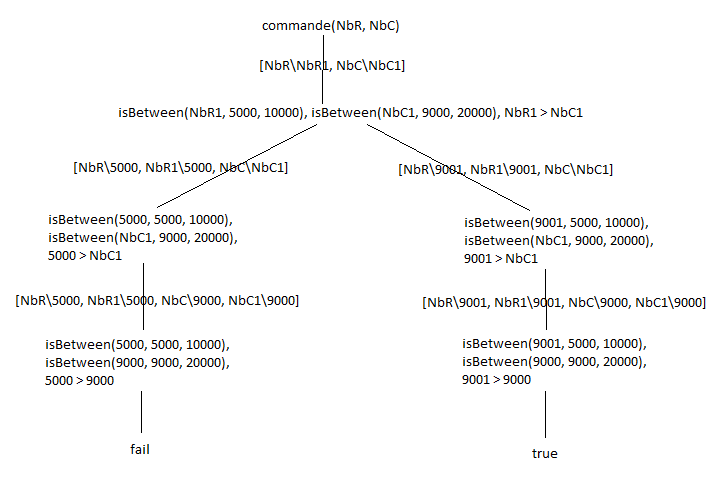
\includegraphics[width=1\textwidth]{searchtree-commande.png}
  \caption{Arbre de recherche de l'exécution du but \textit{commande(-, -)}}
  \label{fig:searchtree-commande}
\end{figure}

\subsection*{Question 1.6}
\textit{Pourquoi peut-on dire que Prolog ne comprend pas les Maths ?}
Si on pose le prédicat $>$ avant les appels à \textit{isBetween} nous obtenons une erreur d'instanciation.
En effet, ECLiPSe ne peut comparer deux nombres qui ne sont pas instanciés.

Nous pouvons dire que Prolog ne comprend pas les maths car il se contente finalement de générer, puis de vérifier, toutes les solutions possibles.
Il n'est donc pas capable de résoudre un ensemble d'équation comme nous le faisons manuellement.

\subsection*{Question 1.7}
Une contrainte est insatisfaisable parce que les contraintes primitives n'ont pas de valeurs fixées.
Le problème peut être résolu en utilisant du \textit{labeling}.

\subsection*{Question 1.8}
La figure \ref{fig:searchtree-labeling} présente l'arbre de recherche Prolog lors de l'exécution du but \textit{commandeLabeling(-NbR, -NbC)} qui utilise cette fois le solveur \textit{ic} avec du \textit{labeling}.
\begin{figure}
  \center
  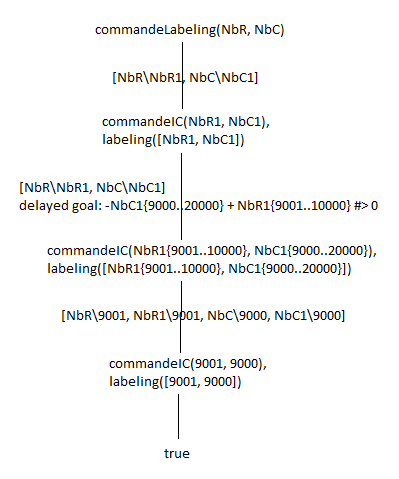
\includegraphics[width=0.5\textwidth]{searchtree-labeling.png}
  \caption{Arbre de recherche de l'exécution du but \textit{commandeLabeling(-, -)}}
  \label{fig:searchtree-labeling}
\end{figure}


\section{Zoologie}

\lstinputlisting[caption=zoologie.ecl]{../zoologie.ecl}
\vspace{2cm}

\subsection*{Question 1.9}
Il faut 3 pies et 14 pattes pour totaliser 5 têtes et 2 chats.

\subsection*{Question 1.10}
Nous trouvons en posant les équations qu'il faut un même nombre de chats et pies pour avoir 3 fois plus de pattes que de têtes.
Cependant, comme on peut le voir lorsqu'on n'effectue pas de \textit{labeling}, le solveur de la bibliothèque \textit{ic} ne semble pas capable d'effectuer cette réduction.


\section{Le OU en contraintes}

\lstinputlisting[caption=ou-constraint.ecl]{../ou-constraint.ecl}
\vspace{2cm}

\subsection*{Question 1.12}
Le calcul de la valeur absolue avec utilisation de l'opérateur de disjonction \textit{or} de \textit{ic} semble s'exécuter beaucoup plus rapidement que l'autre version. Cela semble être dû au fait qu'une plus grande utilisation de contraintes permet une meilleure réduction.

Nous pouvons aussi remarquer que les résultats n'apparaissent pas dans le même ordre malgré que l'ordre des contraintes soit le même.

\end{document}